\documentclass[a4paper, 12pt]{report}
\usepackage[14pt]{extsizes} % для того чтобы задать нестандартный 14-ый размер шрифта
\usepackage[utf8]{inputenc}
\usepackage[russian]{babel}
\usepackage{setspace,amsmath}
\usepackage[left=20mm, top=15mm, right=15mm, bottom=15mm, nohead, footskip=10mm]{geometry} % настройки полей документа
\setlength{\parindent}{5ex}
\setlength{\parskip}{1em}

\usepackage{indentfirst}
\usepackage{geometry}
\usepackage{tikz}
\usepackage{float}
\usetikzlibrary{calc}
\usetikzlibrary{decorations.pathmorphing}
 
\begin{document} % начало документа
 
\begin{titlepage}

\begin{tikzpicture} [overlay,remember picture]
    \draw [line width=0.5mm ] 
		($ (current page.north west) + (1cm, -1cm) $)
    rectangle
    ($ (current page.south east) + (-1cm, 1cm) $);
\end{tikzpicture}

% НАЧАЛО ТИТУЛЬНОГО ЛИСТА
\begin{center}

\hfill \break
\large{Министерство образования РФ}\\
\large{Московский физико - технический институт}\\
\normalsize{2020 - 2021 учебный год}\\ 
\hfill \break
\hfill \break
\normalsize{Физтех - школа радиотехники и компьютерных технологи}\\
\hfill \break
\hfill \break
\normalsize{Реферат по теме:}\\
\hfill \break
\LARGE{«Культура и быт языческой Руси»}\\

\end{center}

\hfill \break

\vspace*{4cm}
\begin{flushright}
  Выполнил: \\
  студент 1 курса \\
  группы Б01-003 \\
  Лепарский Роман Денисович \\
  \hfill \break
  Проверил: \\
  Доц. Департамента истории \\
  Черникова Л.П. 
\end{flushright}
 
\vspace*{1cm}
\begin{center}
	г. Москва (Долгопрудный) \\
	2020 г.
\end{center}

\thispagestyle{empty} % выключаем отображение номера для этой страницы
 
% КОНЕЦ ТИТУЛЬНОГО ЛИСТА

\restoregeometry

\end{titlepage}

\setcounter{page}{2}
 
\newpage
     
    \tableofcontents % Вывод содержания
\newpage
 
\newpage

%===========================================================================================================================================

\chapter*{Введение}
\addcontentsline{toc}{chapter}{\noindent Введение}

В России, как и в любой стране, культура развивалась в тесной взаимосвязи с историей и  религией. Знаменитый отечественный философ Николай Александрович Бердяев выделял в русской истории пять основных периодов, одним из которых является период языческой культуры$^1$\footnote{Источник: https://pagandom.ru/yazychestvo/kul-tura-i-byt-yazycheskoi-rusi.html}. Этот период является одним из самых древних в истории Древней Руси. Его хронология относится к первому тысячелетию н.э.




В 988 году Русь приняла христианство. С того времени прошло уже 11 веков, а так или иначе, ритуалы, восхваляющие силу природы, прочно вошли в наши привычки. Часто, обращая внимание на приметы, отмечая праздники или соблюдая традиции, мы даже не догадываемся, откуда они берут свое начало. Что же сохраняет их силу и влияние? Народная память, хранящая древние обычаи, или скрытая от нашего понимания тайная сила?$^2$ \footnote{https://kulturologia.ru/blogs/130718/39635/}

Точных сведений о божествах и ритуалах славян немного: письменность появилась на Руси лишь в IX веке и распространилась далеко не сразу. До сих пор не найдено ни одного древнерусского документа того времени, который описывал бы верования древних славян. Большинство старинных берестяных грамот посвящены торговле: это частные письма, счета; значительно реже встречаются церковные тексты и фольклорные произведения.
 
Практические все заключения историков основаны на свидетельствах византийцев, германцев и других «гостей» Руси, а также на ряде летописных источников, в которых иногда проскальзывают упоминания обрядов.

Во время археологических раскопок часто находят идолов и ритуальные предметы, но как расшифровать их без текстовых описаний? Ученым остается только делать осторожные предположения$^3$. \footnote{https://www.culture.ru/materials/151806/verovaniya-na-rusi-do-kresheniya} Но одно мы знаем наверняка: славяне свято чтили традиции и поклонялись стихиям. Душа значилась для них главной ценностью, а поклонение божествам — важнейшей составляющей жизни.

Почему меня привлекает данная тема? Меня очень интересует, чем жили, что любили наши предки. В кого верили, кого боялись. Когда я слушаю песни,стилизованные под те времена, хочется узнать, правдивы ли тексты этих песен, действительно ли люди обожествляли силы природы и поклонялись им, какие обряды проводили, какие молитвы использовали.
   
  Откуда на руси появилось язычество? Куда и по какой причине оно пропало? Какой след оно оставило в культурном образе? Существуют ли в современном мире отголоски того периода?
На эти вопросы я постараюсь найти ответ.




\chapter{Зарождение языческой Руси} 

\section{Формирование}

Славянское язычество — система дохристианских представлений о мире и человеке, основанная на мифологии и магии, и связанных с этими представлениями верований и культов древних славян. В целостном виде не сохранилось, реконструируется по данным письменных источников, языка, фольклора, обрядов, обычаев и верований славянских народов$^4$\footnote{https://ru.wikipedia.org/wiki/Славянское\_язычество}.

Как уже говорилось выше, язычество на Руси начало формироваться ещё в первом тысячелетии нашей эры, когда славянские племена начали выделяться из народов индоевропейской группы$^5$\footnote{Источник: https://historykratko.com/slavyanskie-yazycheskie-bogi}.
Вследствие этого процесса, культура Руси того времени имеет немало общих черт с культурами соседних народов. Например, само слово "Бог" для описания образов.
Из германо-скандинавской мифологии языческая Русь переняла концепт мирового дерева, а так же большого количества божеств, которые со временем трансформировались с учетом быта славян.

Стоит упомянуть, что некоторые особенности культуры cлавян могли разниться в зависимости от территориального фактора. Например, культуры восточных и западных славян могли довольно сильно отличаться друг от друга. 


Письменные источники и многие косвенные свидетельства позволяют
нам утверждать, что язычество древних славян было культом
природы. Люди не имели тех знаний, которыми мы обладаем сейчас, а когда у человека нет фактов, он начинает искать причинно-следственные связи. В прошлом году шли дожди, а в этом засуха. Молния попало в дерево. Огненный шар уходит и появляется белый. Почему? Людям были нужны объяснения. 

 Современные исследования позволяют выявить несколько этапов развития язычества.
На первом этапе религиозные представления древних славян были
связаны с обожествлением сил природы, которая представлялась населенной
множеством духов, что отразилось и в символике древнеславянского
искусства. 

Славяне поклонялись матери-земле, символом которой были
узоры, изображающие большой квадрат, поделенный на четыре малых
квадрата с точками в центре - знак вспаханного поля. 

На втором этапе развития древнеславянского язычества складывается
и держится дольше других культ Рода и Рожениц - творца вселенной и
богинь плодородия Лады и Лели. Это был культ предков, семьи и домашнего
очага. Изображения Лады и Лели на многочисленных вышивках продолжали появляться и в XVIII-XX вв.


В это же время складывается и трехчастное представление о мире:
нижнем - подземном, Нави (символ - ящер), среднем - земном,Яви (изображались
обычно люди и звери) и верхнем - небесном, звездном. Прави. Изображение данной
структуры мира можно было увидеть на идолах, сохранившихся лишь в
единичных экземплярах; а также русских прялках, изготовлявшихся еще сто
лет назад.

Поклонения и жертвоприношения проходили в специальных
культовых святилищах-капищах, которые представляли собой
первоначально округлые деревянные или земляные сооружения,
возведенные на насыпях или холмах, а позднее они приобрели
четырехугольную форму.

 Обычно у славян роль храма выполнял лес. Наличие храмовых помещений у славян (за исключением западных) не зафиксировано, однако они вполне могли иметь место, не оставив после себя следов, будучи деревянными. На капище проводились обряды поклонения идолам. Капища могли быть огорожены, их обычным атрибутом был костёр, временный или постоянный. Очевидно, капище было построено князем Владимиром для его пантеона, однако оно до сих пор не обнаружено археологами.

На третьем, завершающем этапе развития язычества появляется культ
Перуна, дружинного бога-громовержца. В 980 г. киевский князь Владимир I,
прозванный Красное Солнышко, предпринял попытку реформировать
язычество, придав ему вид монотеистической религии. Стремясь поднять
народные верования до уровня государственной религии, князь приказал
поставить деревянные идолы шести богов; Перуна с серебряной головой и
золотыми усами, Хорса, Даждьбога, Симаргла и Мокоши. 

Таким образом можно отследить, что славянская религия формировалась на протяжении долгого периода в процессе выделения древних славян из индоевропейской общности народов во II—I тысячелетии до н. э. 


\chapter{Религия}

Религия - это про исповедание веры посредством внешних знаков,про поклонение Высшему. Для чего человеку религия? Она формирует картину мира и место в нём человека, а также систему ценностей. Религия помогает человеку справиться с социальным и психологическим напряжением, успокаивает, приносит облегчение, чувство защищенности и уверенности. 

Во времена дохристианской Руси основной религией было Язычество. Выдержка из Википедии:

Язычество — принятый в христианском богословии и в исторической литературе термин, обозначающий традиционные и нехристианские религии. В более узком смысле, язычество — политеистические религии. Впрочем, далеко не все «языческие религии» политеистичны. Термин язычество происходит из Нового завета, в котором под язычеством подразумевались народы или «языки», противополагаемые ранним христианским общинам$^6$.\footnote{https://ru.wikipedia.org/wiki/Язычество}

Религия языческой руси была как раз политеистической, то есть включала в себя несколько богов, о которых и пойдет речь дальше.

В первом тысячелетии н.э. на Руси не было комплекса сказаний о божествах такого, как например в греческой или скандинавской мифологии. Первый письменный исторический материал - "Повесть Временных лет" датируют XI веком. Поэтому, большинство из того, что мы знаем сейчас о дохристианском пантеоне было получено из устного народного творчества.

\begin{figure*}[h]
	\caption{Реконструкция славянского святилища}
	\begin{center}
	\includegraphics[scale = 0.5]{2.eps}
	\end{center}
\end{figure*} 

\section{Языческий пантеон}
В начале I тыс. н. э. древнеславянские божества принимают
антропоморфную форму. Главными среди них становятся боги солнца, неба, огня, ветра,
богатства,плодородия. Как можно заметить, люди обожествляли то, в чем нуждались. 
Были у этих богов и свои символы в искусстве. Петух, с изумительной
точностью отмечающий время, признавался вещей птицей, и редкая сказка
обходилась без упоминания о нем. Конь, это гордое стремительное
животное, зачастую сливавшееся в представлении древнего славянина то с
богом солнца, то с образом конного воина, был излюбленным мотивом
древнерусского искусства, да и много позже его изображение продолжало
появляться на коньках русских изб и теремов. Особым почитанием
пользовалось солнце, и изображение огненного колеса («громовой круг»),
расчлененного на шесть частей, прочно вошло в изобразительное искусство.
Эти изображения появлялись на наличниках изб и вышитых полотенцах
вплоть до начала XX в.


На сегодняшний день нам известны следующие славянские божества$^5$\footnote{Описание божеств взято с сайта https://historykratko.com/slavyanskie-yazycheskie-bogi}:

Общеславянские боги:

\begin{itemize}
  \item Перун — верховный бог, двойник Зевса и Тора, потому что мечет молнии и также прозывается громовержцем. Он также является покровителем княжеского рода, им клянется княжеская дружина при заключении международных договоров. Упоминается в Повести временных лет, а также Прокопием Кесарийским, который, правда, не называет его прямо, а указывает, что у славян есть бог-громовержец, которому те приносят в жертву быков;
  \item Мать — Сыра Земля — женское олицетворение живородящей, плодородной земли, ей поклонялись, прося хорошего урожая или большого количества детей; существовала также «клятва землей», которая считалась нерушимой.
\end{itemize}

Боги восточных славян (пантеон князя Владимира):

\begin{itemize}
  \item Хорс — о всей видимости бог-солнце. Историки не смогли выяснить происхождение имени этого бога и по нескольким источникам (один из которых агиографический) его отнесли к олицетворяющему солнце. В одном из источников Хорс назван жидовским богом, что может свидетельствовать о том, что он был заимствован из Хазарского каганата, который исповедовал иудаизм. Исследователь русского язычества В. Н. Топоров полагает, что имя Хорса иранского происхождения и перешло в славянский пантеон от скифов и сарматов;
  \item Даждьбог — солнечное божество, считается предком русских людей.Имя его означает "податель всех благ". Даждьбог ездит по небу в чудесной колеснице, запряженной четверкой белых огнегривых коней с золотыми крыльями;
  \item Стрибог — божество, связанное с ветрами;
  \item Симаргл — вестник между небесами и землей;
  \item Мокошь — женское божество, покровительница прядения и ткачества;
  \item Волос — покровитель скота;
  \item Велес — покровитель сказителей и поэзии;
  \item Рожаницы — божества, олицетворяющие судьбу;
  Род - создатель всего сущего. 
  \item Сварог — бог-кузнец,который по легенде дал человечеству огонь и научил ковать металл. Сварог особо почитался крестьянами, поскольку был первым землепашцем: победив огромное чудище – Змея, он на нем пропахал по Днепру заградительную борозду. Появление Сварога в мифологии относят к железному веку, т. е. к праславянской общности.;
  \item Сварожич — олицетворение огня.
\end{itemize}

Боги западных славян$^7$\footnote{Описание божеств взято с сайта https://ru.wikipedia.org/wiki/Список\_славянских\_богов}:

\begin{itemize}
  \item Святовит — главный бог Арконы, связан с войной и победой;
  \item Триглав — главный бог своей местности, с ним связан священный вороной конь, у его идола три головы;
  \item Сварожич (Радегаст) — главный бог земли ратарей, связан с воинскими функциями;
  \item Чернобог — злой бог, приносящий несчастье. Повелитель Нави,Тьмы и Пекельного царства.;
  Белобог - воплощение света,добра и удачи.Святилище его было на холме,открытом солнцу,а многочисленные золотые и серебрянные украшения отражали игру лучей и даже ночью озаряли храм,где не было ни одного мрачного уголка. 
  \item Прове — главный бог округи Старгарда, почитался в священной дубовой роще;
  \item Припегала — бог с неясными функциями, судя по источнику\footnote{Письмо магдебургского архиепископа Адельгольта, 1108 год} — «дионисийского» типа;
  \item Подага — бог вагров с неясными функциями, имевший храм и идол в Плуне;
  \item Жива — женское божество, главное божество своей местности\footnote{Земля полабов}.
\end{itemize}

Мне не удалось найти список божеств южных славян. Возможно, у них были только общеславянские боги и мифо-ритуальные персонажи.

\section{Низшая мифология}

Низшая мифология — сфера мифологических представлений, относящихся к персонажам, которые не имеют божественного статуса, демонам и духам, и противопоставляются высшим богам и официальному культу$^8$.\footnote{https://ru.wikipedia.org/wiki/Низшая\_мифология}

К низшей мифологии принадлежали разные классы неиндивидуализированной, часто также неантропоморфной нечисти, духов, животных. Они были связаны с мифологическим пространством от дома до леса, болота и т. п. Сюда относились домовые, лешие, водяные, русалки, вилы, лихорадки, мары, моры, кикиморы, судички у западных славян; из животных — медведь, волк. 

Персонажи низшей мифологии часто принимают активное участие в жизни людей, встречаются с ними, превращаются в людей и др., поэтому во многих мифологиях эти персонажи имеют большее значение, чем божества, действовавшие, как правило в мифическое время первотворения.

Существа низшей мифологии чаще всего являются персонажами наиболее популярных фольклорных жанров: сказок, быличек и др., тогда как боги представлены в собственно мифологических повествованиях.

К персонажам низшей мифологии принадлежат духи природы — лесные, горные, речные, морские, о духи, связанные с земледелием, плодородием земли, духи растительности, персонификации календарных праздников (славянские Ярила, Герман, итальянская Бефана и др.), образы языческих богов, в неофициальной народной традиции пониженные и замещённые святыми — покровителями плодородия и др. (русские Велес — Власий, Мокошь — Пятница и др.), различные злые духи (нечистая сила), во многих традициях возводимые к падшим ангелам, и др.

В описаниях различных мифологических традиций часто используется понятие демон, заимствованное из греческой и европейской мифологий. Этим словом условно называются сверхъестественные персонажи, занимающие в иерархии низшее место по сравнению с богами или находящиеся на низших уровнях мифологической системы. В более узком и точном смысле демонами именуются злые духи.

Часто персонажами низшей мифологии выступают реальные животные, хотя часто они выступают персонажами высших уровней вплоть до пантеона. На низших мифологических уровнях представляются как духи — покровители различных природных локаций: лесов, полей, гор, ущелий, рек, озёр, морей, болот и др. и как враждебная людям нечисть.

Таким образом, В религии древних славян присутсвовал анимизм - вера в одушевленность природы. Религия древних славян делилась на высшую и низшую мифологию. К высшей относились антропоморфные образы сил природы - Боги, а к низшей - неантропоморфные существа,духи природы - русалки (духи воды) , леший (дух леса), и т.д. 


\chapter{Обряды древних славян}


Непрерывная борьба и поочередная победа светлых и темных сил
природы художественно была закреплена в представлениях славян о
круговороте времен года. Их исходной точкой было наступление нового года
- рождение нового солнца в конце декабря. Это празднование получило у
славян греко-римское название - «коляда». 

Был также обычай ходить с маем
(символом весны) - маленькой елкой, украшенной лентами, бумагой,
яйцами. Божество солнца, провожаемого на зиму, называли Купала, Ярило и
Кострома. Во время праздника весны соломенное чучело этих божеств или
сжигали, или топили в воде.


Языческие народные праздники, вроде новогодних гаданий,
разгульной масленицы, «русальной недели» сопровождались
заклинательными магическими обрядами и были своего рода молениями
богам об общем благополучии, богатом урожае, избавлении от грозы и
града. Для новогоднего гадания об урожае использовались особые сосуды -
чары. На них часто изображались 12 различных рисунков, составляющих
замкнутый круг - символ 12 месяцев.

Характерным древнеславянским обрядом была масленица, сопровождавшаяся катанием огненного колеса, сожжением чучела зимы, кулачными боями и ряженными. Места для молений старались выбирать на возвышенностях – холмах и горах. Там же сжигались чучела зимы и проводились обряды заклинания весны. В равнинных местностях обряды проводили на лугах. К разряду культовых мест относились также священные рощи («рошения») и священные деревья («древеса»). Особо почитаемыми деревьями были берёза и дуб, символ бога Перуна, а также деревья, расположенные вблизи родников и источников.

Календарные праздники и обряды древних славян-язычников имели сельскохозяйственную подоплёку, многие из них к тому же были связаны с культом предков. Считалось, что именно предки, покоящиеся в земле, благословляют будущий урожай, поэтому для обеспечения плодородия древние славяне стремились задобрить покойных родных: на Масленицу их поминали блинами, им посвящали разнообразные соревнования.

Многие языческие обряды, совмещаясь с новыми христианскими верованиями, образовывали своеобразные синкретические формы двоеверия. Например, праздник Коляды был приурочен к Рождественским святкам, проводы зимы (Масленица) — к Сырной неделе, Красная горка и Радуница — к Пасхе, Семик или Русалии — к Троице, Купала — к Иванову дню (Иван Купала). Отправление обрядов сопровождалось пением песен, бóльшая часть которых сохранилась в народной памяти на долгие годы. В модифицированном виде они дожили до наших дней.

Как говорилось ранее, местами поклонений древних славян идолам были открытые святилища – капища. В центре капища стоял идол - главный объект культа славян-язычников. Эти скульптурные изображения божеств, довольно примитивные по исполнению, могли быть как деревянными, так и каменными. Существует мнение, что в Северо-Западной Руси роль святилищ могли играть сопки – насыпи над захоронениями.

В языческий период у славян были распространены два вида посредников между народом и богами — жрецы, отправлявшие культ в святилищах, и волхвы, имевшие много других названий (ведуны, чародеи, маги, ворожеи и пр.). Последние играли у славян большую роль. Действуя без храмов, помпы и жертвоприношений, волхвы оказывали значительное влияние на верования народа, их жизнь.В IX–X столетиях на Руси сложилась влиятельная прослойка волхвов. Под их руководством проводились обряды, ими сохранялась мифология и разрабатывалась символика. Даже простому волхву надо было знать и помнить все обряды, ритуальные песни, заговоры, уметь вычислять календарные сроки магических действий, знать целебные свойства трав Основной удар христианская церковь направляла против языческой магии, потому что языческих богов она уничтожила сразу. Волхвования же и колдуны оставались, и церковь вела с ними упорную борьбу, которая часто оказывалась безрезультатной. 

После крещения Руси волхвы стали постепенно терять влияние, однако этот процесс не был быстрым: с одной стороны, летописи фиксировали случаи «избиения» волхвов, с другой – даже спустя сто лет после крещения Руси происходили ситуации, когда в противостоянии с князем или епископом волхвов поддерживали целые города. Так было, например, в 1071 году в Новгороде.

\begin{figure}[H]
\begin{center}
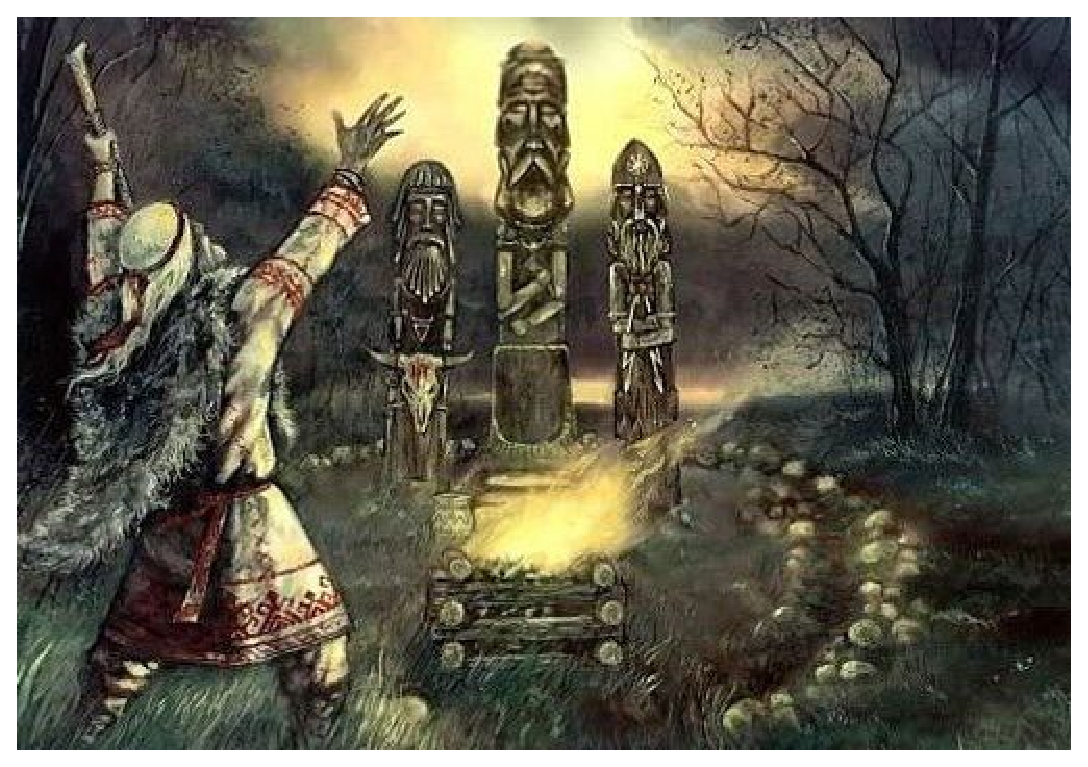
\includegraphics[scale = 0.5]{idol.eps}
\end{center}
\end{figure}

Таким образом, языческие обряды,которые в наше время носят лишь развлекательный характер, раньше имели глубокий, символический смысл.

\chapter{Язычество в культуре и фольклоре} 

Фольклор является самым богатым источником для исследователей славянской мифологии. Сказки, былины, обрядовые песни, заговоры, несомненно, содержат отголоски древних мифов. Проблема состоит в том, чтобы установить, насколько эти отголоски соответствуют самим мифам, в какой мере можно на основе фольклорных данных реконструировать славянскую мифологию.

Известно, что чем большее число посредников участвует в передаче информации и соответственно чем дольше она идет по цепи передатчиков, тем больше вероятность ее искажения. Это относится и к передаче мифов. Когда миф сохраняется с древнейших времен в записанном виде, обеспечивается его передача с минимальными искажениями. Небольшое число издержек наблюдается и в том случае, если миф передается как сакральное знание, вплетенное в ритуал. Славяне же до крещения были бесписьменными, и мифы послужили основой для многочисленных сказок, былин, песен, заговоров.

Такие жанры фольклора, как обрядовые песни и заговоры, сохранили мифологическое содержание с меньшими искажениями, чем остальные. А произошло это потому, что обрядовые песни и заговоры остались в контексте ритуала (того самого языческого ритуала, который жестоко преследовался христианской церковью и тем не менее сохранялся на уровне народных обрядов, обычаев и суеверий).


К наиболее древним обрядовым песням относятся колядки, исполняемые во время зимнего солнцестояния (24 декабря), — праздника Коляды или Овсеня. К этому празднику рождения нового солнечного года был приурочен христианский праздник Рождества. Сохранившийся поныне обычай колядовать восходит к древним языческим обрядам, связанным с аграрно-магическими действиями: гаданием, предсказанием приплода, посыпанием зерном, ряженьем, пожеланиями урожая в новом году и достатка 15. Обряд колядования включал величания хозяину дома, его семье. Такие колядки пели с припевом "Святый вечер".

Довольно часто встречается другой припев — "коляда", "колиодка" или "коляда-маляда" — с таким припевом исполнялась одна из древнейших колядок, отражающая древний языческий ритуал, "За рекой огонь горит".

Самый полный вариант текста этой песни был записан в 30-е гг. XIX в.:

\begin{center}
	За рекою, за быстрою, \\
	Ой, колиодка! Ой, колиодка!\\
	Леса стоят дремучие.\\
	Во тех лесах огни горят,\\
	Огни горят великие,\\
	Вокруг огней скамьи стоят,\\
	Скамьи стоят дубовые,\\
	На тех скамьях добры молодцы,\\
	Добры молодцы, красны девицы,\\
	Поют песни колиодушки.\\
	Ой, колиодка! Ой, колиодка!\\
	В середине их старик сидит,\\
	Он точит свой булатный нож.\\
	Котел кипит горючий,\\
	Возле котла козел стоит;\\
	Хотят козла зарезати.\\
\end{center}

Несомненно, в тексте этой колядки сохранились воспоминания о древнем обряде; по-видимому, здесь идет речь о языческом жертвоприношении, которое сопровождается обрядовой культовой песней с упоминанием Коляды (колиодка).
Как видим, славянская дохристианская мифология очень богата и разнообразна. Благодаря этногорафическим изысканиям сегодня мы можем воссоздать быт и культуру наших предков во всем многообразии и многоцветии фольклорных традиций, ремесел, былин, сказаний и обрядов. Можно сказать, что фольклорная традиция – это зеркало жизни Древней Руси.

Хотя, например, Е.В. Аничков\footnote{Евгений Васильевич Аничков — русский историк литературы, критик, фольклорист, прозаик.}, считал язычество в Древней Руси «убогим», славянских богов «жалкими», а нравы «грубыми». И действительно, если сравнивать мифы и легенды славян с богатейшей мифологией Древней Греции или Скандинавии, то сравнение будет не в пользу Руси. Языческие русские обряды и в самом деле очень примитивны, но зато древнерусский фольклор может считаться одним из самых многозначительных. Б.А. Рыбаков\footnote{Борис Александрович Рыбаков — советский и российский археолог, исследователь славянской культуры и истории Древней Руси}, чтобы опровергнуть точку зрения Аничкова, провел серьезнейшие исследования по древнерусской языческой мифологии и, можно сказать, «доказал», что и мы не хуже, и наше язычество может быть поэтичным и всеобъемлющим.

В целом древнерусская фольклорная традиция и связанные с ней обряды и обычаи имела тесные связи с земледельческим календарем. Смена времени года рассматривалась нашими предками, как борьба холода и тепла, символическая смерть и возрождение.

Были у древнерусского язычества и свои жрецы, их называли волхвы и приписывали им магическую силу и власть. Уже после христианизации Руси волхвы пытались вернуть себе власть в умах жителей, однако, их попытки, получившие в истории название «восстания волхвов», провалились. В XI веке мятежные волхвы объявляются то в Новгороде, то в Киеве, иногда народ и князья принимают их сторону, иногда волхвов «избивают».

Сам феномен волхва, волховства – сквозной сюжет славянской фольклорной традиции. Вспомним смерть Вещего Олега от коня, напророченную волхвами, легенду о Всеславе Полоцком, который был рожден не от любви, но от волхования (колдовства), волхвы предсказывают победы и поражения русских князей. Характерно, что волхвы борются с ведьмами, обвиняя их в том, что они прячут урожай или насылают засуху, голод и болезни (мор). Для того, чтобы снять проклятие ведьму следовало убить и вырезать у ней из живота каравай хлеба или рыбину, после этого бедствия отступали. Священники как могли боролись с этими жестокими обычаями, волхование было объявлено ересью и, таким образом, поставлено вне закона.

Самым известным феноменом в русской фольклорной традиции являются, конечно же, былины. Они как героический эпос зародились именно в Древней Руси, а может быть и ранее, с приходом к власти князя с дружиной.

Существует много теорий относительно происхождения былины как жанра, в современной науке сумма этих теорий признается как правильная. То есть былины - это и сказания  в которых богатыри (своего рода двойники славянских богов) борются с напастями (силами природы) и выходят из них победителями; в былинах также мы видим и отголоски реальных исторических событий, романтизированных последующими пересказчиками и переписями; безусловно, некоторые былины или их элементы были заимствованы из фольклора западных и восточных соседей. Таким образом русские былины – сложный феномен, в зависимости от того, кто обращается к его изучению (историк, литературовед, лингвист), раскрываются те или иные его грани. 

С точки зрения истории, безусловно, в былинах нашли отражение реальные исторические события. «Слово о полку Игореве», былины Владимирова цикла, Задонщина - базируются на реальных фактах, нашедших свое подтверждение в официальной науке. В связи с этим былинный эпос получил статус исторического фольклора.

В развитии былинного эпоса можно выделить две большие стадии. Первая – это зарождение былины как жанра, собственно языческий период. В былинах этого цикла действуют почти мифические герои-богатыри. Они олицетворяют силы природы и обладают не просто физической, но сверхъестественной силой. Таким нам рисуется великан Святогор, которого не держит Мать-Сыра-Земля, Микула Селянинович – дохристианский богатырь-пахарь, бросивший вызов Святогору. Дочь Микулы – Василиса является сквозным женским персонажем во всем русском былинном эпосе. Вольга Святославич – еще один древнейший персонаж былин, он может обращаться в разных животных и «читает по книгам». 

После древнего периода былин выделяют еще два – киевский и новгородский, образовашиеся уже после крещения Руси и поэтому не относящиеся как таковые к древнерусскому язычеству. В киевском цикле богатыри-герои группируются возде фигуры Владимира Красное Солнышко (скорее всего поэтического образа реально существовавшего князя Владимира), в новогородском цикле действуют Садко, Василий Буслаев.

Важно особенностью древнерусского язычества является его всепроникающий характер, а также сохранение «двоеверия» на протяжении всей истории нашей страны. Обряды, заклинания, амулеты и гадания остались в нашей культуре и по сей день, языческая семиотика прочно вошла в православную традицию несмотря на многочисленные запреты церковных деятелей, раздававшиеся уже в первые годы после крещения Руси.

Огромно влияние, которое оказало язычество на русскую литературу: былины, сказки, обрядовые песни прослеживаются практически во всех произведениях классической и современной русской литературы. К языческим истокам обращались в своем творчестве Пушкин, Гоголь, Платонов и даже Маяковский.

 Таким образом,языческая традиция Древней Руси сыграла и продолжает играть огромную роль в развитии всей русской культуры.

\chapter{Закат язычества}

Своего рода религиозный дуализм установился на Руси задолго до Владимира. В христианизации Руси была заинтересована Византия, где считалось, что любой народ, принявший христианскую веру из рук императора и константинопольского патриарха, автоматически становится вассалом империи. Контакты Руси с Византией способствовали проникновению христианства в русскую среду. На Русь был послан митрополит Михаил, крестивший, по преданию, киевского князя Аскольда. Христианство было популярно среди дружинников и купеческой прослойки при Игоре и Олеге, а княгиня Ольга и вовсе сама стала христианкой во время визита в Константинополь в 950-х годах. В период самостоятельного правления князя Святослава, с первой половины 960-х годов по 972 год, христианство стало гонимой религией, поскольку Святослав был убеждённым язычником.

По летописной легенде, крещению Владимира предшествовал осознанный выбор им веры. Князь и его окружение якобы выслушали \\миссионеров-представителей разных конфессий: булгар-мусульман, «немцев из Рима», хазарских иудеев и «философа-грека из Византии». Тогда Владимир разослал в разные страны своих соратников, чтобы те посмотрели и узнали, какая вера лучше, и те, возвратившись, сказали – нет веры лучше греческой. На деле, как полагают исследователи, принятие христианства было во многом продиктовано прагматическими соображениями: новая вера должна была обеспечить религиозно-идеологическое подкрепление государственности и власти киевских князей.

Крещение Владимира стало лишь отправной точкой для христианизации всей Руси: тысячелетнее язычество медленно отступало под натиском духовенства, и сам процесс растянулся на многие десятилетия. При Владимире крестились только княжеские семья и дружина, в чьих рядах и до 988 года было немало адептов христианства. Основная масса населения оставалась языческой в XI веке, да и в начале XII века, как писал один из сводчиков, вятичи ещё «творили» языческие обряды. 

Археологические находки показывают, что языческие обряды и празднества и прикладное искусство с языческой символикой в большей или меньшей степени котировались у жителей древнерусских городов вплоть до середины XIII века, не говоря уже о деревнях, где христианизация протекала гораздо медленнее. В полной мере отождествляли себя с христианством только представители третьего поколения после крещения Руси, жившие в эпоху Ярослава Мудрого.



Письменная традиция на Руси имела своей целью определить место новой, только что народившейся государственности в христианской цивилизации, а потому выметала с книжных страниц все, что противоречило православию. Всем этим было, в первую очередь, язычество, с его «погаными» баснями и героями, Церковь называла их «кощунами». 

Таким образом, христианизация Руси была не гуманной и противоречила всем нормам этики. В конечном итоге, церковь так и не смогла искоренить язычество. Приурочивание языческих праздников к церковным, сохранившиеся и передающиеся из поколение в поколение песни и обряды всегда напоминали людям о родной Вере.

\chapter*{Заключение}
\addcontentsline{toc}{chapter}{\noindent Заключение}

Несмотря на многочисленные запреты, языческие черты проникли в православную традицию и укоренились в системе русских традиций и обычаев. К самым известным примерам относятся празднуемые и ныне Масленица, Иван Купала, Святки, Чистый четверг, проводы зимы. Огромные костры над могилами – пережитки языческих трупосожжений – в некоторых местностях фиксировались вплоть до конца XIX века. Из языческих времён в современность перекочевали многие календарные обряды и сельскохозяйственные приметы, огромный пласт фольклора.

Если раньше поклонение языческим богам требовало определенных церемониалов, жертвоприношений и обрядов, то с момента крещения Руси, оно утратило свою сакральность и осталось в повседневности в виде забав, сказов, басен, игр молодежи, гаданий и т. п. В таком, можно сказать, непринужденном виде язычество сохранилось до настоящего времени, оказывая влияние на разивтие всей русской культуры и продолжает его оказывать до сих пор.

\chapter*{Список использованных источников}
\addcontentsline{toc}{chapter}{\noindent Список использованных источников}
 
\begin{enumerate}
	\item https://pagandom.ru/yazychestvo/kul-tura-i-byt-yazycheskoi-rusi.html
	\item https://kulturologia.ru/blogs/130718/39635/
	\item https://www.culture.ru/materials/151806/verovaniya-na-rusi-do-kresheniya
	\item https://ru.wikipedia.org/wiki/Славянское\_язычество
	\item https://historykratko.com/slavyanskie-yazycheskie-bogi
	\item https://ru.wikipedia.org/wiki/Язычество
	\item https://ru.wikipedia.org/wiki/Список\_славянских\_богов
	\item https://ru.wikipedia.org/wiki/Низшая\_мифология
\end{enumerate}
 
\end{document}